%-----------------------------------------------------------------------------
%
%               Template for sigplanconf LaTeX Class
%
% Name:         sigplanconf-template.tex
%
% Purpose:      A template for sigplanconf.cls, which is a LaTeX 2e class
%               file for SIGPLAN conference proceedings.
%
% Author:       Paul C. Anagnostopoulos
%               Windfall Software
%               978 371-2316
%               paul@windfall.com
%
% Created:      15 February 2005
%
%-----------------------------------------------------------------------------


\documentclass[preprint]{sigplanconf}

% The following \documentclass options may be useful:
%
% 10pt          To set in 10-point type instead of 9-point.
% 11pt          To set in 11-point type instead of 9-point.
% authoryear    To obtain author/year citation style instead of numeric.

\usepackage{amsmath}
\usepackage{syntax}
\usepackage{url}
\usepackage{graphicx}
\usepackage{qtree}
\usepackage{multicol}
\usepackage{times}

\begin{document}

\conferenceinfo{PPOPP '12}{date, City.} 
\copyrightyear{2011} 
\copyrightdata{[to be supplied]} 

\titlebanner{DRAFT}        % These are ignored unless
\preprintfooter{draft version}   % 'preprint' option specified.

\title{Towards Parallel and Distributed Programming using Bottom-Up Logic Programming}

\authorinfo{Flavio Cruz \and Ricardo Rocha}
           {CRACS \& INESC-Porto LA, Faculty of Sciences, University of Porto\\
                  Rua do Campo Alegre, 1021/1055, 4169-007 Porto, Portugal}
           {\{flavioc,ricroc\}@dcc.fc.up.pt}
\authorinfo{Michael Ashley-Rollman \and Seth Copen Goldstein}
           {Carnegie Mellon University, Pittsburgh, PA 15213}
           {\{mpa,seth\}@cs.cmu.edu}

\maketitle

\begin{abstract}
In the last few years there as been a steady increase of processing power.
Multicore processors are now increasingly prevalent and networks of commodity computers
present an opportunity to solve more challenging problems. Programming in these kinds of
systems is not as simple as it should be since optimizing programs to run on
different types of distributed systems is notoriously hard.
We propose a logic programming language based on Datalog
that is suitable for developing general purpose programs for
both parallel and distributed systems. The language uses the notion of
link restricted rules for parallelizing computation
and \emph{action facts} for doing input/output.
We developed a compiler and a runtime system with several execution strategies,
from multithreaded execution to distributed execution using MPI. We also
developed several techniques based on XY-stratification to reduce memory usage
and increase parallelism. We present several application cases, from graph
problems to machine learning algorithms, that show that our language is
suitable to take advantage of parallel architectures.
\end{abstract}

\category{CR-number}{subcategory}{third-level}

\terms

\keywords

\section{Introduction}

The last decade has seen a priority shift for processor companies. If clock frequency
was once the main metric for performance, today computing power is measured in number of
cores in a single chip.
For software developers and computer scientists, once focused in developing sequential programs,
newer hardware usually meant faster programs without any change to the source code. Today,
the free lunch is over. Multicore processors are now forcing the development of
new software methodologies that take advantage of increasing processing power through parallelism.
However, parallel programming is difficult, usually because programs are written
in imperative and stateful programming languages that make use of relatively low level synchronization
primitives such as locks, mutexes and barriers. This tends to make the task of managing multithreaded
execution quite intricate and error-prone, resulting in race hazards and deadlocks.
In the future, \emph{many-core} processors will make this task look even more daunting.

On the other hand, advances in network speed and bandwidth are making distributed computing
more appealing. For instance, \emph{cloud computing} is a new emerging paradigm that wants
to make every computer connected to the Internet as a client of a pool of computing power,
where data can be retrieved and computation can be done. From the perspective of high performance
computing, the \emph{computer cluster} is a well established paradigm that uses fast local area
networks to improve performance and solve problems that would take a long time with a single computer.

Developments in parallel and distributed programming have given birth to several programming models.
At the end of the spectrum are lower-level programming abstractions such as
\emph{message passing} (e.g., MPI~\cite{gabriel04-open-mpi}) and \emph{shared memory}
(e.g., Pthreads and OpenMP~\cite{Chapman-2007-UOP-1370966}).
While such abstractions are very expressive and enable the programmer to write very performant code,
they tend to be very hard to use and debug, due to synchronization problems, making it difficult to
prove the program's correctness.

An approach that attempts to address the correctness challenges, is to use declarative languages
such as \emph{logic programming languages} or \emph{functional programming languages}. In logic languages such
as Prolog, researchers took advantage of the non-determinism of proof-search to evaluate subgoals
in parallel with models such as \emph{or-parallelism}~\cite{ali-86} and \emph{and-parallelism}~\cite{Shen-92}. In functional languages, the stateless nature of computation
allows multiple expressions to evaluate safely in parallel. This has been explored in several languages
such as NESL~\cite{Blelloch:1996:PPA:227234.227246} and Id~\cite{Nikhil93anoverview}.

Recently, there has been an increasing interest in declarative and data-centric languages.
MapReduce~\cite{Dean:2008:MSD:1327452.1327492}, for instance, is a popular data-centric programming
model that is optimized for large clusters. The scheduling and data sharing model is very simple:
in the \emph{map phase}, data is transformed at each node and the result reduced to a final
result in the \emph{reduce phase}.

A declarative approach that is becoming popular is Datalog~\cite{Ullman:1990:PDK:533142}, a
bottom-up logic programming language.
Traditionally used in deductive databases, Datalog is being increasingly used in different fields
such as distributed networking~\cite{Loo-condie-garofalakis-p2}, sensor
nets~\cite{Chu:2007:DID:1322263.1322281} and cloud computing~\cite{alvaro:boom}.

In the context of the Claytronics project~\cite{goldstein-computer05}, a massive distributed system,
we've been using a Datalog variant called Meld~\cite{ashley-rollman-iclp09, ashley-rollman-derosa-iros07wksp}.
Meld is specially suited for writing programs for distributed systems where the network
topology can change dynamically. Such systems are called \emph{ensembles} and they include
programmable sensor networks and modular robotic systems.

Lately, we have been adapting Meld to implement general parallel algorithms in multicore machines
and clusters. We are using the concept of \emph{action facts} to model output and the language
has been extended with lists, aggregate modifiers, and new methods for source code analysis to
reduce deletion and improve throughput.

We have implement a new compiler and a virtual machine that is able to execute on multicore machines
and distributed networks. For multicore machines we have implemented different scheduling schemes,
including static division of work and work stealing.
For distributed networks and clusters we are using MPI with a static division of work.
Finally, the runtime system is also able to take advantage of multicores when doing distributed computation,
thus we can execute programs on multicore clusters, using several threads on the same process to speedup
computation.

The rest of the paper is organized as follows. In the next section we describe the Meld language
and the modifications we made to make it more suitable for parallel programming. Next, we present
how the runtime system distributes the computation across processors and machines and the different
scheduling schemes. In Section~\ref{sec:evaluation} we evaluate the language modifications with
several applications from graph theory and machine learning. Finally, we end the paper outlining
some conclusions and future work.

\section{The Meld Language}

Meld is a bottom-up logic programming language based on Datalog. Like Datalog, its
execution consists in a database of \emph{facts} plus a set of \emph{production rules} for generating new facts.
Each fact is an association between a \emph{predicate} and a tuple of values. A predicate can be seen
as a relation or table in which the tuples are its elements. Production rules have the form
$\mathtt{p :- q_1, q_2, ..., q_n.}$, logically meaning that "if $\mathtt{q_1}$ and $\mathtt{q_2}$ and ... and
$\mathtt{q_n}$ are true then $\mathtt{p}$ is true".

\subsection{Evaluation}

When a Meld program starts executing, the set of initial axioms in the form $\mathtt{p.}$ are
instantiated and added to the database. With these new facts, rules are then fired and new
facts are generated and added to the database, until a \emph{quiescent} state is reached, where
no more facts can be generated. In Meld, we can also have \emph{action facts},
which are syntactically similar to regular facts but cause some side effect. In the context of
modular robotics, action facts activate the robot's actuators in order to produce movement
or control devices. For parallel programming we use the concept of action facts for writing
results to files or to the terminal. Note that action facts are not added to the database.

\subsection{Rules}

A Meld program contains a set of rules. A rule has two main components: the \emph{head},
which indicates the facts to be generated; and the \emph{body}, which contains the pre-requisites
to generate the head facts. The body may contain the following as pre-requisites: \emph{subgoals},
expression constraints or/and variable assignments. The head can only contain subgoals.
Variables are limited to the scope of the rule and must be defined in the body subgoals or through
the body variable assignments. Variables that only appear on the head are forbidden, since each
instantiated fact must have only \emph{ground facts} and thus all arguments must be instantiated.
The abstract syntax for the language is presented in Fig.~\ref{fig:definitions}.

\newcommand{\synlineend}{\\[.5ex]}
\begin{figure}
\small
\begin{tabular}{lrl}
Structural Facts & $\Gamma ::=$ & $\cdot \| \Gamma,f(\hat t)$  \synlineend

Sensing Facts & $\Theta ::=$ & $\cdot \| \Theta,f(\hat t)$ \synlineend

Accumulated Actions & $\Psi ::=$ & $\cdot \| \Psi,a(\hat t)$  \synlineend

Set of Rules & $\Sigma ::=$ & $\cdot \| \Sigma,R$ \synlineend

Actions & $A ::=$ & $a(\hat x)$ \synlineend

Facts & $F ::=$ & $f(\hat x)$ \synlineend

Constraints & $C ::=$ & $c(\hat x)$ \synlineend

Assignments & $A ::=$ & $e(\hat x)$ \synlineend

External Functions & $X ::=$ & $f(\hat x)$ \synlineend

Expression & $E ::=$ & $E \wedge E \| F \| C \| A \| X$ \synlineend

Rule
& $R ::=$ & $E \Rightarrow F \| E \Rightarrow A \| agg(F, g, y) \Rightarrow F$ \synlineend
\end{tabular}
\vspace*{-1ex}
\caption{Abstract syntax for Meld programs}
\vspace*{-2ex}
\label{fig:definitions}
\end{figure}

Whenever all body pre-requisites are satisfied, the head subgoals are instantiated as
facts and then they are added to the program database (except when action facts are derived).
To satisfy all pre-requisites, the body
subgoals must be matched against the program database. Both constraints and subgoals
match successfully when a consistent substitution is found for the body's variables such that one or
more facts in the database are matched. Constraint expressions are boolean expressions that
use variables from subgoals (and thus database facts) and from variable assignments. Allowed
expressions in constraints include arithmetic, logical and set-based operations.

Each predicate used in the program must be explicitly typed. Each field is either of a basic
type or a structured type. Basic types include the integer type, floating point numbers and
the \emph{node address} (see \ref{sec:localization}).
A structured type includes lists of basic types. Syntax-wise, lists have a syntax similar to Prolog.

\subsection{Aggregates}

In contrast to Datalog, Meld does not have negation, but has \emph{set aggregates}
\footnote{It has been shown in~\cite{zaniolo-arni-ong-dood93} that set aggregates can be
implemented using negation, however we implement aggregates directly, without using source
code transformation.}. The purpose of an aggregate is to define a type of predicate that combines
the facts of that predicate into a single fact. The definition of an aggregate includes the
field of the predicate and the type of operation to be done on the collection of facts.

Consider a predicate $\mathtt{p(f_1, ..., f_{m-1}, agg\ f_{m}, f_{m+1}, ..., f{m+n})}$,
where $f_m$ is the aggregate field associated with the operation $\mathtt{agg}$. For each
combination of values $\mathtt{f_1, ..., f_{m-1}}$ there will be a set of facts matching
the same combination. To calculate the aggregated fact of each collection, we take all
the $\mathtt{f_{m}}$ fields and apply the $\mathtt{agg}$ operation. The fields between
$\mathtt{f_{m+1}}$ and $\mathtt{f_{m+n}}$ for the aggregated fact are chosen depending
on the operation.

Meld allows several aggregate operations, namely: \texttt{max}, to compute the maximum value;
\texttt{min}, to compute the minimum value; \texttt{sum}, to sum all the values of the corresponding
fields; and \texttt{first}, to select the first fact field.

\subsection{Localization}\label{sec:localization}

Another difference between Meld and Datalog, is that in the former, the first field
of each predicate must be typed as a node address.
In rules, the first argument of each subgoal is called the \emph{home variable} and
refers to a place, called the \emph{node}, where facts are stored.
Therefore, each node has its own database.

This convention originated in the context of declarative networking~\cite{Loo-condie-garofalakis-p2},
namely, in the P2 system. For modular robotics, this makes it trivial to
distribute data across the ensemble. In the context of this paper, each fact is a
\emph{structural fact} and can be seen as part of the data structure representing a node in the graph.
Moreover, when each fact is associated with a certain node, it helps us distribute
and parallelize computation and also improve data locality (see~\ref{sec:topology}).

While each fact must be associated with some node, a rule may contain subgoals that refer to
different nodes. In order to simplify the activation of production rules, each rule is transformed so that
each subgoal refers to the same node. The process of \emph{localization} is fundamental
in the distribution of computation.

Before localization, each rule can be either a \emph{local rule} or a \emph{link-restricted rule}.
A local rule does not need to be transformed since only facts from a single node are needed.
A link-restricted rule is a rule where subgoals may refer to different nodes. This type of rule
must be transformed so that the right subparts of the rule are matched
on the right nodes (by matching the facts of that node only)
and the instantiation of the head subgoals into facts is done on the subgoal the head subgoals
refer to. To accomplish this, the nodes involved in the computation of the rule must communicate
between each other so that the rule is fired when everything has been known to match.
For this, we introduce a special class of facts called the \emph{link facts}. These facts
represent the edges in the graph and force the nodes to do direct communication with
only their direct neighbors.

For an example, consider the following block of Meld code, where a rule refers to three different
nodes, \texttt{A}, \texttt{B} and \texttt{C}.

\begin{verbatim}
fact2(A, 2) :-
   fact1(A, A1), A1 > B1,
   edge(A, B), fact1(B, B1), B1 > C1,
   edge(A, D), fact1(D, D1),
   edge(B, C), fact1(C, C1).
\end{verbatim}

To localize this rule, we first build a tree representing the connection paths between nodes by
picking an arbitrary root node, in this case, the node \texttt{A}, and then by adding
edges using link facts. The resulting tree is represented in Fig.~\ref{fig:loctree}.
Note how the constraints were placed in the bottom-most node where all the variables used in the constraint
were available. This optimization aims to reduce communication by testing constraints as soon as
possible.

\qtreecenterfalse
\begin{figure}[ht!]
\scalebox{0.70}{
\Tree [.{\bf A} [.{\bf B} [.{\bf C} {\tt fact1(C, C1)} ] {\tt{fact1(B, B1),}\\$\mathtt{B1 > C1}$} ] [.{\bf D} {\tt fact(D, D1)} ] {\tt fact1(A, A1),\\ {\tt A1 $>$ B1}} ]
}
\caption{Localization tree}
\label{fig:loctree}
\end{figure}

Once connection paths are known, localization transforms the original rule into several
\emph{send rules}, that are characterized by having the same node in the body and a different
node in the head. Once a send rule body matches,
all the subgoals in the head are instantiated and then sent to the corresponding node,
where the matching of the original rule can continue, until the complete rule matches.
The following code shows the final result.

\begin{verbatim}
__edge(X, Y) :- edge(Y, X).

fact2(A, 2) :-
   fact1(A, A1), A1 > B1,
   __remote1(A, B1), __remote3(A).
   
__remote1(A, B1) :-
   __edge(B, A), fact1(B, B1), B1 > C1,
   __remote2(B, C1).
__remote2(B, C1) :-
   __edge(C, B), fact1(C, C1).
__remote3(A) :-
   __edge(D, A), fact1(D, D1).
\end{verbatim}

\subsection{Pipelined Evaluation}

Evaluation of Datalog programs (including programs with recursive rules) can be done using
several techniques, one of the most well-known being the \emph{semi-naive fixpoint}
evaluation~\cite{Balbin1987259, Bancilhon:1986:NER:8789.8804}. However, these techniques
are more appropriate for a centralized evaluation and are expensive in a distributed environment,
because they require global synchronization. To this end, we use the \emph{pipelined semi-naive}
evaluation from P2~\cite{Loo-condie-garofalakis-p2}, which relaxes the semi-naive fixpoint
by making the concept of iteration local to a node.

Whenever a new fact is generated by the node or sent by a neighbor node, the fact is added to local
queue which contains all new facts. As execution proceeds, a fact is pulled out of the queue. Then,
all rules that use the fact in their body are selected as \emph{candidate rules}. For each candidate, the
rest of its rule body is matched against the facts in the database. If the rule is proved, the subgoals
in the head of the rule are instantiated and added to the local queue as new facts.

\subsection{Example: Shortest-Path}

For an example, consider the program in Fig.~\ref{fig:shortestpath} that computes the
shortest distance and the corresponding path between any node to node 4.
Each edge in the graph is represented
by the \texttt{edge} relation in \texttt{r4}, and includes the source node, the destination node and
the distance of the connection. Note how node addresses are prepended with the symbol @.

\begin{figure}
\begin{verbatim}
type end(node).
type route edge(node, node, int).
type path(node, min int, list node).

r1: path(A, W, [A, B]) :-
      edge(A, B, W),
      end(B).

r2: path(A, D + W, [A | P]) :-
      edge(A, B, W),
      path(B, D, P).
  
r3: write_int(A, W), write_list(A, P) :-
      terminated(A),
      path(A, W, P).
  
r4: edge(@0, @1, 1). edge(@1, @2, 1).
    edge(@2, @3, 3). edge(@0, @2, 4).
    edge(@2, @0, 2). edge(@1, @4, 2).

r5: end(@4).
\end{verbatim}
\caption{Shortest Path in Meld}
\label{fig:shortestpath}
\end{figure}

The \texttt{path} predicate is a transitive closure
subject to an aggregated field, which forces the selection
of the fact with the least distance. In \texttt{r1}, we define the path
for each neighbor node of node 4, by declaring that a node \texttt{A} has an edge to node \texttt{B}
and node \texttt{B} is the selected final node.
In \texttt{r2} we complete the transitive closure, declaring that the shortest path between \texttt{A}
and a node \texttt{B} is the sum of the distance between \texttt{A} and \texttt{B} and the
shortest distance between \texttt{B} and node 4.

\begin{figure}[ht]
  \centering
    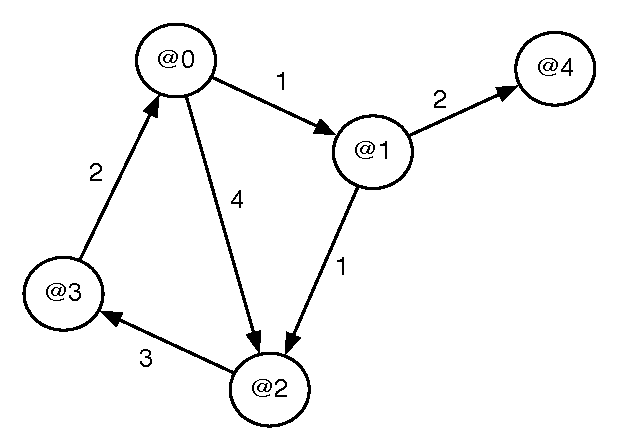
\includegraphics[width=0.28\textwidth]{figures/shortestpathgraph.pdf}
  \caption{Shortest path graph.}
  \label{fig:shortestpathfig}
\end{figure}

Using the localization method, we know that node 4 will send a fact representing
a match of rule r1 to its neighbors, in this case, node 1. Node 1 then instantiates a new
path fact \texttt{path(@1,~2,~[@1, @4])}. At this moment, node 1 could generate the aggregated
\texttt{path} fact representing the least path to node 4 or could wait until all the \texttt{path}
facts are generated.

In a distributed setting, it is difficult to assess if all facts of an
aggregate collection are already on the database (we present techniques to avoid this in XXX).
However, we use a technique borrowed from P2 called \emph{deletion} that allows Meld
to retract facts derived from invalid facts such as aggregates based on partial information
or changes in the environment (in the case of modular robotics). Deletion
is presented in detail in the next section.

In this case of example graph (Fig.~\ref{fig:shortestpathfig}), node 1 can generate the least path
safely and send it to node 0. Node 0 receives this fact and generates a new aggregate: \texttt{path(@0,3,[@0,@1,@4])}. Node 0 then sends a new fact to node 3. Then, node 3 generates a
new aggregate and instantiates a new fact that is sent to node 2. Node 2 then generates its
least path aggregate: \texttt{path(@2,8,[@2,@3,@0,@1,@4])} and fires rule r2 for neighbors
node 0 and node 1. However these new paths are not minimal and thus nothing is generated,
resulting in a fixpoint in the graph. If, however, a better path was found, everything
derived from the old path would have to be deleted and the new path added to the database.

After the fixpoint is reached, a new fact, \texttt{terminated} is generated for each node
and rule r3 is activated, which forces the writing of the minimum distance and the shortest path
to the terminal. The \texttt{terminated} fact is called a \emph{sensing fact}, since it is not
part of the node data structure, but is associated with the state of execution. 

\subsection{Deletion}

Deletion is mechanism that allows Meld to delete all facts derived from invalid facts such
as aggregates based on partial (and incomplete) information. In modular robotics,
deletion is used to delete everything derived from old world information and thus keep the database
of facts consistent to the robot's environment.

Deletion works by considering a deleted fact and matching the rules in exactly the same way as
derivations are done to determine which facts depend on the deleted one. Care must be taken when
deleting facts that were derived by different rules. To accomplish this, we use a reference counting
scheme similar to garbage collection techniques. We
keep track of the number of derivations of the fact and, optionally, the
the depth of derivation of the fact.

The reference count is incremented or decremented whenever the fact is derived or
deleted, respectively. When the reference count reaches zero, we delete the fact and anything
derived from it. The derivation depth is used for facts that have cyclic derivations so that
no infinite cyclic derivations are left with no start.
This mechanism is throughly explained in~\cite{ashley-rollman-iclp09}.

\subsection{Aggregates and Recursive Rules}

\subsubsection{XY-Stratification}

\cite{zaniolo-arni-ong-dood93}

\subsubsection{Aggregate modifiers}

Aggregate modifiers 

\section{Parallel Execution}

Distributing the execution of Meld programs is relatively easy since our compiler automatically
transforms the original program into fully distributed code. Due to the language semantics,
messaging and placement of data is pre-defined which helps distribute execution.

In our execution model, we have the set of nodes in the graph and a set of \emph{workers}.
A worker is an independent unit of processing and it is usually either a \emph{thread} or
a \emph{process}. A worker can process new facts at most from one node at the same time and
a node can be handled at most by one worker at the same time. This restriction simplifies
parallelization by not allowing several works to manipulate the database of a node at the same time.

The main task of our runtime system is thus to balance the load between workers, so that we
can maximize the speedups. However, we need to make a distinction between \emph{monotonic}
facts (non-aggregates) and \emph{non-monotonic facts} (aggregates). The former maximizes
distribution, while the latter requires some form of synchronization in order to
minimize deletion of facts. Note that doing computation with the wrong fact and the fact
that workers compute in a non-deterministic manner, it makes the completion process highly
non-deterministic, since many facts can be wrongly derived and then deleted and recomputed,
everything depending on how the order of processing of workers.

In order to make evaluation deterministic for any set of workers,
the distributed evaluation procedure of Meld programs is as follows:

\begin{itemize}
   \item Workers process all monotonic facts (i.e., non-aggregates) and no aggregates are fired,
   except if they can be generated \emph{safely};
   \item When a worker does not have more work, it enters into the \emph{idle state}.
   \item Once the graph reaches a quiescent state, that is, when all workers are in
   the idle state, all workers synchronize through a \emph{termination barrier};
   \item Upon synchronization, aggregates are then generated using the facts of each
   aggregate collection;
   \item If any new fact was derived (or a deletion is to be done), they are added to the
   corresponding queues, and we start a new \emph{computation round};
   \item If no new facts were derived, the computation is marked as complete and finishes.
\end{itemize}

Parallelization is maximized when the number of global synchronizations required to compute
the whole program is minimized. Making the generation of aggregated facts a local decision
at the node level thus contributes to increased asynchronicity between nodes and increased
throughput of the whole system.

In the remaining subsections we describe several optimizations and scheduling strategies
of our runtime system.

\subsection{Topology Ordering}\label{sec:topology}

For certain scheduling schemes that will be presented shortly,
to distribute computation across workers it is important
to increase locality of communication, so that a node makes most of its communication to
neighbor nodes that are being handled by the same worker. This means that the data travels
in the same worker, which can potentially increase performance. If a worker is a process,
this means that less inter-process communication or network communication will be done, and,
in the case of a thread, it may mean more data locality and cache hits.

Our compiler is able to know how many nodes are in the graph and, in most cases, all the
edges of the graph. This is detected by analyzing the node address constants (that are prepended
by the symbol @) and the axioms of the program. After parsing and type-checking the program code,
the compiler then optimizes the topology by building an internal representation of the graph.
In this phase, each node address $a$ is mapped using a function $M(x)$ to a normalized node
address $n$. Function $M(x)$ is bijective and the domain is the set of all nodes described in the
source code. The codomain of $M$ is the discrete interval $[0, N[$, where $N$ is the number
of nodes in the graph. The byte-code of a Meld program includes all the pairs $(x, M(x))$ so
that the runtime system can put this information to use.

We have two methods for defining the function $M(x)$:

\begin{itemize}
   \item \emph{Randomized}: the mapping is done randomly.
   \item \emph{Breadth-First}: the mapping is built by picking an arbitrary node, $n_{zero}$
   and setting $M(n_{zero}) = 0$, then we select all neighbors of $n_{zero}$ and start defining
   their mappings in increasing order, 1, ..., $N-1$, and adding its neighbors for later processing
   in a breadth first fashion.
\end{itemize}

The breadth-first method is used with the intent of clustering closer nodes in an ordered fashion.
While not optimal, using a breadth-first approach is very efficient and has good results for
irregular graphs. If we use a static division of work between $N$ workers, where each worker
is responsible to process a pre-defined set of nodes, we can efficiently slice the domain of function
$M(x)$ and divide it between the $N$ workers.

For an example, consider the graph in Fig.~\ref{fig:topology1}. The node addresses represented
are the ones included in the source code. Using a breadth-first method starting by node 1,
we get the following order: 1, 2, 3, 7, 5, 6 and 4. If we had to do a static division of worker
for 2 workers, worker 1 would get 1, 2, 3, 7 and worker 2 would get 5, 6 and 4. Note from
Fig.~\ref{fig:topology1} that only 3 edges exist between the nodes of worker 1 and worker 2.
This greatly reduces communication between workers and improves parallel efficiency.

\begin{figure}[ht]
  \centering
    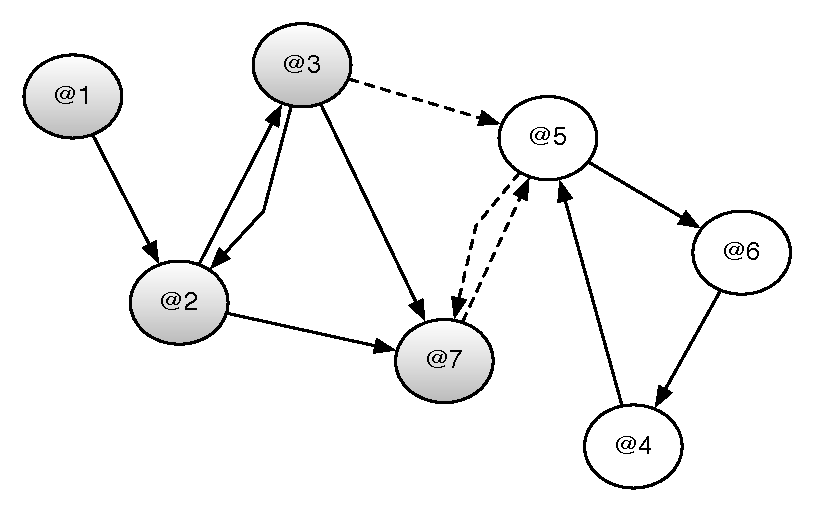
\includegraphics[width=0.35\textwidth]{figures/topology1.pdf}
  \caption{Topology using a breadth-first method.}
  \label{fig:topology1}
\end{figure}

We intend to explore other methods for defining $M(x)$ in the future, such as the METIS
partitioning method~\cite{Karypis:1998:FHQ:305219.305248}.

%\subsection{Selective Localization}

\subsection{Scheduling}

We implemented several \emph{scheduling schemes} to distribute computation across workers.
Most of these methods are dependent on the nature of the worker in order to maximize efficiency.
We present results for several programs in Section~\ref{sec:evaluation} using the schedulers
described here to assess how the scheduling scheme improves or degrades the speedup.

We previously said that each node had a queue of new facts to process. However, this can be relaxed
in order to account for the existence of workers. We have been experiencing with two main different
types of queue organizations for parallel and distributed computation: local and global queues.

\subsubsection{Local Queues}

In the local queues organization, each node has a local queue of facts to process and
there is one or multiple queues of \emph{active nodes} to handle.
An active node is a node that contains new facts to process and must be handled by some worker.

In Fig.~\ref{fig:localqueues} we present a schematic of local queues. For each local queue
we have new facts which are represented the \texttt{predicate}, the \texttt{tuple} and the
\texttt{count}. The \texttt{count} field is an integer and is used to distinguish between
derivations and deletions.

\begin{figure}[ht]
  \centering
    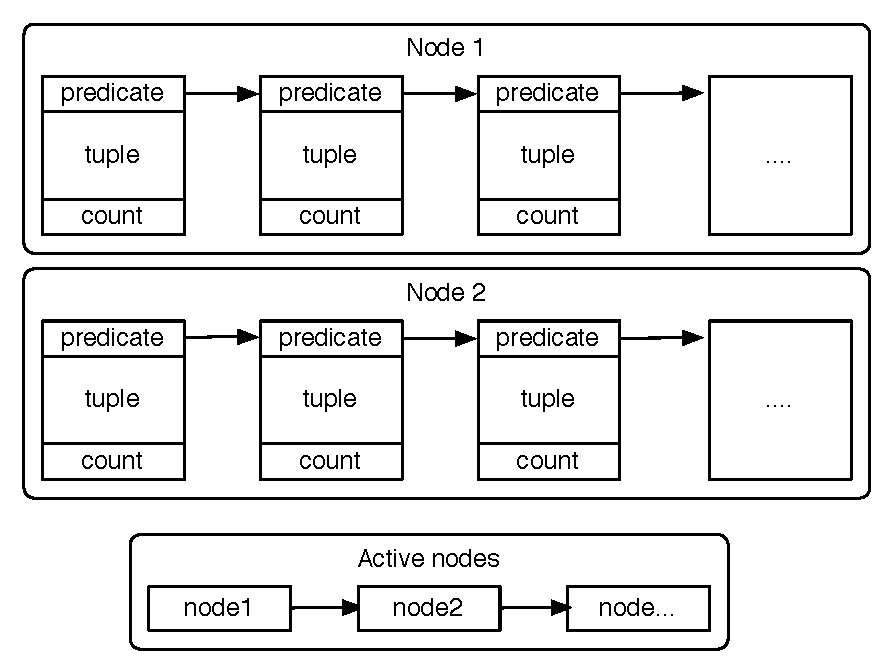
\includegraphics[width=0.35\textwidth]{figures/localqueues.pdf}
  \caption{An example of local queues.}
  \label{fig:localqueues}
\end{figure}

\subsubsection{Global Queues}

In the global queues organization, there is one or more queues with facts to process
and the nodes have no queues themselves. Figure~\ref{fig:globalqueue} presents a
global queue with the fields for each element of the queue. Note that now each queue element
also has a \texttt{node} field, which corresponds to the node the fact is related to.

\begin{figure}[ht]
  \centering
    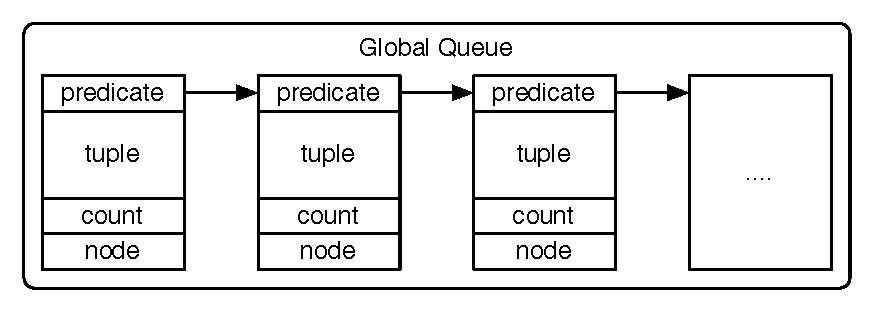
\includegraphics[width=0.35\textwidth]{figures/globalqueue.pdf}
  \caption{An example of a global queue.}
  \label{fig:globalqueue}
\end{figure}

\subsection{Multithreaded Scheduling}\label{sec:multithreading}

Our virtual machine supports multithreaded execution using Pthreads. The workers in all the
following four scheduling schemes are realized as threads.

\subsubsection{Global Static Division (TGSD)}

The \emph{Global Static Division (TGSD)} is a scheduling strategy where each thread
has a global queue and a pre-defined set of nodes $S$ to handle. Every fact that is added
to the global queue must be from a node the thread actually owns.

How is node ownership defined? Using the topology ordering defined previously, we divide
statically the $N$ nodes in the graph across $T$ threads. Because execution
always refers to mapped node addresses, sometimes we must know what thread is responsible for a given
node address. For a node with address $n$, we compute $min(n / (N/T), N-1)$ to know
the corresponding thread number.

Threads use their global queues to pop a new fact and node and then trigger new derivations.
A new fact for a node owned by the same thread is simply added to the thread's queue.
A new fact for a node not owned by the executing thread is, instead of inserted directly
into the corresponding thread's queue, put into a buffer, so that when this buffer reaches
a certain size, we can push the whole buffer directly into the other thread's queue.
This helps improve data locality by making threads not touching other's threads cache lines very often.

Threads enter into the idle state when their global queues are empty. While idle, threads
busily check for new work and for round termination. After the end of each round,
aggregates are generated. Each thread is responsible to generate the aggregates of all
nodes in $S$.

\subsubsection{Local Static Division (TLSD)}

In this scheme, a static division of work is made using the topology ordering. However,
we use local queues instead. Each thread has now a queue of active nodes, where nodes with new
facts to process are put, so that each node's queue can be processed by the thread.
Note that node ownership is exactly the same as TGSD.

Every node that is in the thread's queue has is state defined as \emph{active}.
Threads use their queue of nodes to pop a node to handle. During the \emph{handling} phase,
the thread processes each node's fact until the node's queue is empty, when the node state is then
set from \emph{active} to \emph{inactive}. When a new fact is generated and pushed into
the node's queue, the executing thread checks the target node state. If its \emph{inactive},
it is set as \emph{active} and the node is pushed into the corresponding thread queue in
order to be handled in the future.

In this scheme, threads also enter into the idle state when their queues are empty. When
idle, threads busily check for new active nodes and for round termination. Generation of
aggregates is done in the same way as in TGSD.

\subsubsection{Local Dynamic Division (LDD)}

Local Dynamic Division (LDD) is a scheme where each thread starts with a pre-defined set
of nodes as in the TLSD scheme but gets more dynamic as time goes by.
For instance, when a thread $T1$ enters into the idle state, it
selects a random thread $T2$ to add a \emph{steal request} to the \emph{steal set} of $T2$.
A steal set is a queue of steal requests. A steal request is just a pointer to a
\emph{demanding thread}.
The steal set is processed whenever the thread is going to process more work. First, the thread
pops a steal request from the steal set and checks if there is some active node in the node queue
of the thread. If there is, an active node is popped from the queue and changes ownership
to the demanding thread. In our VM, we can actually change the number of active nodes
to move, so that more work can be pushed faster to other threads.

We could have used a different scheme for work stealing, namely, to force the demanding thread
to steal the active nodes directly from the target thread. However, we opted to create the
steal set, since it will be less accessed than the queue of nodes and therefore will reduce
cache line invalidation. The queue of nodes
is accessed much more frequently, to pop nodes or to add new active nodes, respectively.
The steal set is only modified when a thread enters into the idle state. Furthermore, the design
of the queue of active nodes can be made more efficient since there are multiple pusher threads
and only one thread popping nodes and thus no locking is needed while popping nodes. 

Finally, to generate aggregates, each thread maintains a \emph{node set}, a set of nodes owned
by the thread. For determining the owner of a node during execution of remote rules, each node
has the field \texttt{owner} which points to the corresponding thread.

\subsubsection{Local Dynamic Division without Ownership (LDDWO)}

While the previous scheduler offers substantial dynamism using work stealing,
for certain programs, however, this may lead to nodes keep changing from one thread
to another, hurting performance since the node set needs to be adjusted.
We have developed the \emph{Local Dynamic Division
without Ownership (LDDWO)} scheduler that adds more dynamism and eliminates node ownership
altogether so that any thread can process any node as long as the node is active and is
not being processed by another thread.

In LDDWO each node has a local queue and there is only one queue $Q$ of active nodes for all threads.
To get work, a thread pops a node from $Q$ a processes all its facts. When $Q$ is empty,
threads enter into the idle state.
During aggregate generation, we use a static division as presented previously, where each node
processes aggregates for a pre-defined set of nodes.

The advantages of LDDWO is that a thread can pick up a new node immediately after it becomes active,
improving load balancing and throughput.
However this mechanism offers much less data locality than before since threads can process any node
and not a particular set of nodes. Also, contention on the $Q$ may also degrade performance.

\subsection{Distributed Scheduling}\label{sec:distributed}

Our virtual machine supports distributed scheduling using OpenMPI~\cite{gabriel04-open-mpi},
a low-level message passing library. Contrarily to the previous section, where the worker was
a thread working in a shared memory environment, the worker is now a process working with
other processes.

Processes can be executed on the same machine, in a cluster or in a network of machines.
Because of this, we must take into account for the slower communication time between
processes. We focused mainly on developing static schedulers
and we do not consider dynamic approaches in this paper, since they would require
the movement of nodes between processes, which can be quite expensive since we would
need to move entire databases of facts over the network.

The marshaling of objects is another important aspect of distributed computation. We marshal both
the predicate identifier (\texttt{predicate\_id}), the tuple fields and the derivation/deletion
mark (\texttt{count}). The predicate identifier is an unsigned integer that identifies the predicate
and is common for all processes executing the same program. Each tuple field is marshaled according
to its type. Lists are marshaled recursively as pairs. An example of the fact \texttt{path(2, [@3, @4]))} is presented in Fig.~\ref{fig:marshal}.


\begin{figure}[ht]
  \centering
    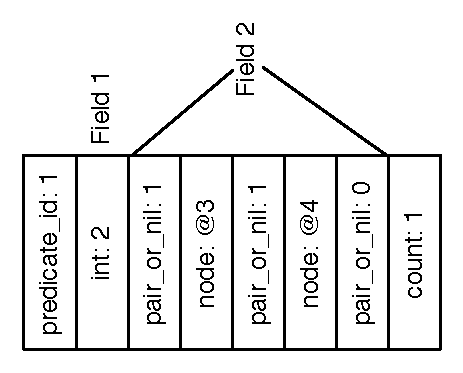
\includegraphics[width=0.25\textwidth]{figures/marshal.pdf}
  \caption{Marshaled representation of the fact \texttt{path(2, [@3, @4])}.}
  \label{fig:marshal}
\end{figure}

When a process fires a remote rule and needs to send a fact to a node in another process, the
fact is added to the corresponding \emph{message set} of the target process. The message set
is a list of messages (or facts) that are being buffered for later sending. When the marshaled
message set reaches an arbitrary size (in this case, the OpenMPI message limit), all the facts
in the message set are sent to the process as a whole to be demarshalled on the other side.
This buffering mechanism helps us reduce the number of communications between processes.

Buffered messages may also be sent periodically, even if the message size limit was not reached.
In the idle state, processes immediately send pending messages and then enter into a busy wait
cycle, where they check for incoming messages or for round termination.

An interesting implementation problem that affects performance is deciding how messages should be sent.
We send the messages in an asynchronous manner, so that processes can send messages through the
MPI subsystem and then continue immediately to process more facts, instead of waiting for 
the completion of the send operation. However, we need to check periodically if the messages
were received in the other end so we can free the allocated memory used for sending, since we cannot
free this memory while MPI is using it.

We have a \emph{request handler} for each process that
maintains a queue of \emph{requests} for each process. A request is a pair containing a memory pointer
and a MPI request handler. Since the queue of requests is ordered by the send time, with the
older messages at the beginning and newer messages at the end, we take the first $N$ MPI handlers
from the first $N$ requests and execute the \texttt{MPI\_Testall} function to test if the
$N$ requests have all been received by the other process. If they were, we free the first $N$ pointers
of memory and then we increase $N$ to $N'$ and try to complete the next $N'$ requests, until
the process fails. We ignore the other requests since if older messages were not received, this
probably means that newer messages were not received yet. The number of tested requests is adapted
dynamically, so that more or less requests are tested at the same time.

The process of sending a new fact to a node in the same process is dependent on the scheduling
scheme used. We may use the \emph{Distributed Global Static Division (DGSD)} scheme,
where each process uses a global queue or the \emph{Distributed Local Static Division (DLSD)} scheme,
where local queues are used.

During the termination of each round, all processes generate their node's aggregates and then
execute a cooperative reduce operation to assess if any of the processes has more work to do,
i.e., if any aggregate value was generated. The reduced value is used
to terminate the computation or start another round.

\subsection{Mixed Mode Scheduling}

Our virtual machine can also mix the two previous means of computation, distributed and multithreaded,
in order to execute several threads in the same MPI process. We still use the static division of
work between different processes, however, we can use the several ways of distributing computation
between threads presented in~\ref{sec:multithreading}.

When a thread interacts with a thread in the same process, all the multithreading rules apply,
however if the other thread resides in a different process, the rules presented 
in~\ref{sec:distributed} will apply, except for a few cases.

Each thread maintains
a message set per target process and is able to send messages and check if the messages were received.
However, only the \emph{leader thread} (an unique thread per process) is able to receive
messages. The leader thread checks for incoming messages and then adds the facts to the
corresponding threads in the same process.
Another role of the leader thread is to work with other threads to detect termination of the
current round (details in~\ref{sec:distributedtermination}). The leader thread thus represents
the whole process and tells the other leader threads when the threads in their process have finished.
However, the leader thread mechanism has a few disadvantages since the time spent receiving messages
can lead to load imbalances.

In a nutshell, we have the following scheduling schemes:

\begin{itemize}
   \item \emph{Mixed Global Static Division (MGSD)}: TGSD is used to manage threads.
   \item \emph{Mixed Local Static Division (MLSD)}: TLSD is used to manage threads.
   \item \emph{Mixed Dynamic Division (MDD)}: LDD is used to manage threads. Threads can steal work from the threads in the same process.
   \item \emph{Mixed Dynamic Division without Ownership) (MDDWO)}: LDDWO is used to manage threads. Threads do not have ownership of the process nodes.
\end{itemize}

\section{Virtual Machine Details} 

In this section we present several details about our VM,
from the byte code instructions, memory management, data structures to detection
of round termination.

\subsection{Byte Code}

The byte code contains the nodes in the graph, the predicate information and the code for
each predicate that implements pipelined evaluation. Axioms are fired by a special predicate
that is instantiated for each node at the beginning of execution.

Each thread or process executes an instance of the VM and all instances can access the common
byte code in memory, however they have their specific data, such as 32 registers, the node they
are executing on and other information.
Instructions range from send instructions, to arithmetic instructions, the cons/head/tail triplet,
conditional instructions and move instructions. A special instruction uses hashing to efficiently
execute certain blocks of instructions for a particular node (such as instantiating axioms).

\subsection{Memory}

In multithreading applications, the memory allocator used can affect the parallel performance.
Our allocator uses multiple pools of objects that are particular to each thread. This helps reduce
contention in memory allocation.

\subsection{Queues}

We employ different queues according to the scheduler used. For the local queues scheme,
where each thread has a queue of nodes to process, 
there is only one thread taking things from the queue and multiple threads adding
things. For this case, the queue used is the \emph{Safe Multiple Pushers Queue (SMPQ)}, which
is a lock-free data structure implemented using a sentinel node,
where CAS (compare and set) instructions are only used during the push operation. SMPQ was adapted
from work done in~\cite{m.michael:simple}.

For queues of facts, namely on nodes or in the global queues scheme, we use a two level data structure.
On the first level we use a \emph{Binary Tree Bounded Priority Queue
(BTBPQ)}~\cite{Shavit94diffractingtrees}, where each priority
level is the stratification level. The BTBPQ is a lock-free binary tree where each leaf is a another
queue for the second level. The second level uses a SMPQ for the facts of the corresponding
stratification level.

Finally, we also have a \emph{Safe Multiple Operations Queue (SMOQ)}, where we can have multiple
threads taking and inserting things in the queue in a thread-safe way using a mutex.
This queue is used for the LDDWO schedulers.

\subsection{Lists}

Our lists are implemented as typical head/tail pairs. Each pair contains the head, the tail and a reference
count field for counting the number of data structures pointing to this pair. The reference counter
is an atomic integer and is incremented when a pair or a field points to it and decremented when
the parent pair is deleted or a tuple is deleted. When the counter reaches zero, the pair is
effectively deleted and the memory freed.

Because Meld enables external function calls we need an extra mechanism to handle nested calls
for functions that return lists, so that intermediate lists are effectively garbage collected.
For each VM instance, we keep a list of created pairs during the execution of a rule. When the
execution of a rule completes, we iterate over the list and check if the reference counter is
still zero. This means that the pair is not being used by any fact, so we delete the pair.
If the pair is connected to other pairs, they may be also be deleted. 

\subsection{Detecting Parallel Termination}

When threads exhaust the work they have to do, they enter into the idle state. Here, we must 
have a way to detect when all the threads have finished, so that we can terminate the current
round. We adapted the work presented in~\cite{Flood:2001:PGC:1267847.1267868} to implement
a termination detection barrier. It includes an atomic counter representing the number
of active threads and a boolean flag for each thread representing the current thread state.
The termination condition is fired when the counter reaches zero.

\subsection{Detecting Distributed Termination}\label{sec:distributedtermination}

We use the famous Dijkstra-Safras token-ring based algorithm~\cite{safras87} for detecting
termination. In this algorithm, there is one leader process that starts with a token. This
token then navigates through all processes until it reaches again the leader process. If
the final balance of sent and received messages on the token is zero and the token is \emph{clean}
(i.e., the token did not stop in a process that was still working) then the round terminates.

\section{Evaluation}\label{sec:evaluation}

In this section we present several programs written Meld that show possible
uses of the language.

\subsection{All-Pairs Shortest Path}

\subsection{PageRank}

\subsection{Belief Propagation}

\subsection{Neural Networks}

\section{Conclusions and Further Work}

\acks

% We recommend abbrvnat bibliography style.

\bibliographystyle{abbrvnat}

% The bibliography should be embedded for final submission.

\bibliography{refs}

\end{document}
